\documentclass[border=3pt,tikz]{standalone}
\usepackage[utf8]{vietnam}
\usetikzlibrary{calc,angles,intersections,shapes.geometric,arrows,decorations.markings,arrows.meta,patterns.meta,patterns}
\usepackage{tikz-3dplot,pgfplots}
\pgfplotsset{compat=1.15}
\usepgfplotslibrary{polar}
\usepackage{amsmath}
\begin{document}

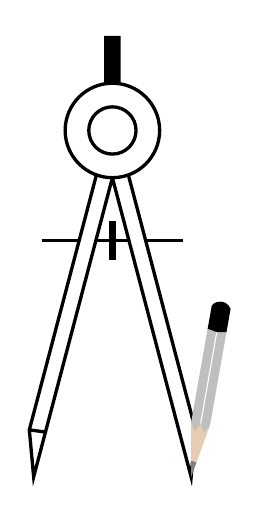
\begin{tikzpicture}
	\coordinate (Diemdat) at (0,0);
	\coordinate (Diemquay) at (2,0);
	\coordinate (a) at ($(Diemdat)!.5!(Diemquay)$);
	\coordinate (b) at ($(a)!5cm!90:(Diemquay)$);
	\coordinate (c) at ($(a)!.88!(b)$);
	\coordinate (m) at ($(Diemdat)!.6!(b)$);
	\coordinate (n) at ($(Diemquay)!.6!(b)$);
	\path[name path=ac] (a)--(c);
	\path[name path=mn] (m)--(n);
	\path[name path=circlec] (c) circle (.6);
	\path[name intersections={of= ac and circlec,by=x}];
	\path[name intersections={of= ac and mn,by=y}];
	\draw[line width=6pt] (b)--($(c)!2!(b)$);
	\draw[very thick] ($(y)!.9cm!90:(c)$)--($(y)!.9cm!-90:(c)$);
	\draw[line width=2.5pt] ($(y)!.25cm!90:(n)$)--($(y)!.25cm!90:(m)$);
	\filldraw[fill=white, draw=black, very thick] (x)--($(x)!.85!(Diemdat)$)coordinate(z)--(Diemdat)--($(Diemdat)!.6cm!20:(x)$)coordinate(t)--($(x)-(Diemdat)+(Diemdat)!.6cm!20:(x)$)--cycle (x)--(Diemquay)--($(Diemquay)!.6cm!-20:(x)$)--($(x)-(Diemquay)+(Diemquay)!.6cm!-20:(x)$)--cycle (z)--(t);
	\filldraw[fill=white, draw=black, very thick] (c) circle (.6cm) (c) circle (.3cm);
	\fill[gray,rotate around={-10:(Diemquay)}] (Diemquay)--++(80:.2)coordinate(a)--++(180:.07)--cycle;
	\fill[brown!40,rotate around={-10:(Diemquay)}] (a)--++(80:.5)coordinate(b)--++(180:.243)--++(-80:.5)--cycle;
	\fill[gray!50,rotate around={-10:(Diemquay)}] (b)--++(-120:.1215)--++(120:.1215)coordinate(m)--++(-120:.1215)--++(120:.1215)--++(90:1.2)coordinate(c)--++(-10:.1234)coordinate(n)--++(10:.1234)coordinate(d)--cycle;
	\draw[white,rotate around={-10:(Diemquay)}] (m)--(n);
	\fill[black,rotate around={-10:(Diemquay)}] (d)--++(90:.3) arc (30:150:.14)--(c)--(n)--cycle;
\end{tikzpicture}

\end{document}